\begin{graphicspathcontext}{{./chapters/mas/architectures/imgs/},{./chapters/mas/architectures/imgs/auto/},{./chapters/mas/imgs/auto/},\old}

\sidenote{\cite{Craig1988}, Image Claude Sonnet 4.6}
\begin{frame}[t]{Motivation for Blackboard Architecture}
	\begin{columns}
		\begin{column}[t]{.1\linewidth}
			\vspace{-.5cm}
			\begin{bottomarrowsequence}[width=1.5cm]
				\arrow[bg=CIADmagenta]{\tiny\hfill Coordination\hfill\mbox{}\newline Problem}
				\arrow[bg=CIADdarkgreen]{\tiny Solution}
			\end{bottomarrowsequence}
		\end{column}
		\begin{column}[t]{.9\linewidth}
			Multiple specialized agents must collaborate to solve a complex
			problem:
			\begin{itemize}
			\item They speak \emph{different languages} (knowledge representations)
			\item No single agent has the \emph{full picture}
			\item The order of contribution is \emph{not known in advance}
			\item Direct peer-to-peer wiring creates \emph{combinatorial coupling}
			\end{itemize}
			\vspace{.1cm}
			\begin{columns}
				\begin{column}[t]{.5\linewidth}
					Introduce a \emph{shared, structured memory} visible to all agents --- the \emph{blackboard}
				\end{column}
				\begin{column}[t]{.5\linewidth}
					\raisebox{-.5\height}{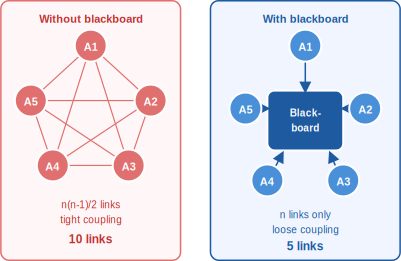
\includegraphics{blackboard_motivation}}
				\end{column}
			\end{columns}
		\end{column}
	\end{columns}
\end{frame}

\sidenote{\cite{Craig1988}, Image Claude Sonnet 4.6}
\begin{frame}{Core Components}
	\begin{columns}
		\begin{column}{0.5\linewidth}
			\begin{definitionblock}{Blackboard}
				A \emph{global, structured data store} partitioned into \emph{levels of abstraction}.
				Agents read from it and write partial solutions back to it
			\end{definitionblock}
			\begin{definitionblock}{Knowledge Sources (agents)}
				Autonomous, specialised modules.
				Each agent monitors the blackboard and \emph{fires} when its trigger conditions are met
			\end{definitionblock}
			\begin{definitionblock}{Coordinator (agent)}
				Decides \emph{which agent runs next}, based on the current state of the blackboard and an opportunistic scheduling strategy
			\end{definitionblock}
		\end{column}
		\begin{column}{.5\linewidth}
			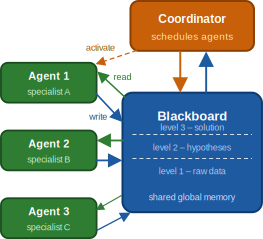
\includegraphics{blackboard_components}
		\end{column}
	\end{columns}
\end{frame}

\sidenote{\cite{Craig1988}, Image Claude Sonnet 4.6}
\begin{frame}{Blackboard Structure}
	\begin{columns}
		\begin{column}{.5\linewidth}
			Blackboard is \emph{vertically partitioned} into levels of abstraction, from raw data at the bottom to high-level solutions at the top\\[.25cm]
			\begin{itemize}
			\item Each level holds \Emph{partial hypotheses} of one abstraction degree
			\item Agents read \emph{across} levels and write their contributions to the \emph{appropriate} level
			\item Solution \Emph{emerges} as information propagates upwards through the levels
			\end{itemize}
		\end{column}
		\begin{column}{.5\linewidth}
			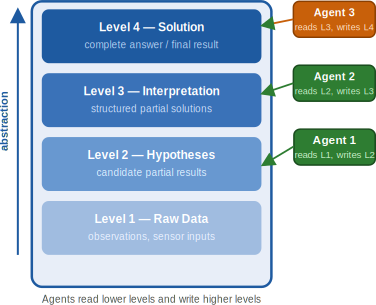
\includegraphics{blackboard_levels}
		\end{column}
	\end{columns}
\end{frame}

\begin{frame}{Interaction Cycle}
	\begin{columns}[T]
		\begin{column}{.5\linewidth}
			\smaller
			System operates as a \Emph{sense–decide–act loop}:
			\begin{enumerate}
			\item \Emph{Monitor}\\
			Each agent observes the blackboard for trigger conditions
			\item \Emph{Evaluate}\\
			The control component scores all ready agents and selects the most promising one
			\item \Emph{Execute}\\
			The selected agent reads relevant entries, computes a partial result, and \Emph{writes} it back
			\item \Emph{Update}\\
			New data may trigger further agents, continuing the cycle
			\end{enumerate}
		\end{column}
		\begin{column}{.5\linewidth}
			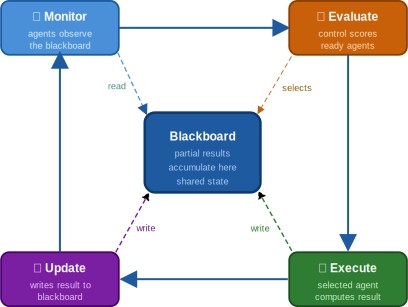
\includegraphics{blackboard_cycle}
		\end{column}
	\end{columns}
\end{frame}

\sidenote{Image Claude Sonnet 4.6}
\begin{frame}{Properties of the Blackboard Architecture}
	\hiconbox{\smaller
		\begin{compactdescription}
		\item[Loose coupling] agents communicate only through the blackboard; no direct links needed
		\item[Incremental solving] partial results accumulate until a complete solution is formed
		\item[Flexibility] agents can be added, removed or replaced independently
		\item[Opportunism] the control component can exploit the most promising partial result at any time.
		\end{compactdescription}
	}{pros-icon}
	\hiconbox{\smaller
		\begin{compactdescription}
		\item[Bottleneck] the blackboard is a single shared resource; concurrent access must be managed
		\item[No guaranteed order] the solution path is emergent and hard to predict
		\item[Scalability] a very large blackboard can become costly to monitor
		\item[Debugging] emergent, opportunistic behaviour is difficult to trace and reproduce
		\end{compactdescription}
	}{cons-icon}
\end{frame}

\end{graphicspathcontext}

\endinput
